%\definecolor{rainbow1}{rgb}{0.5019608f0, 0.0f0, 0.5019608f0}
%\definecolor{rainbow2}{rgb}{0.0f0, 0.0f0, 1.0f0}
%\definecolor{rainbow3}{rgb}{0.0f0, 0.5019608f0, 0.0f0}
%\definecolor{rainbow4}{rgb}{1.0f0, 0.64705884f0, 0.0f0}
%\definecolor{rainbow5}{rgb}{1.0f0, 0.0f0, 0.0f0}

\newcommand\pararealU[2]{\draw (2*#2*\xshift,0) +(\yangle:2*#1*\yshift) node (U#1#2) {$U_{#1}^{#2}$};}
\newcommand\pararealG[2]{\draw (2*#2*\xshift,0) +(\yangle:2*#1*\yshift+\yshift) node (G#1#2) {$G(U_{#1}^{#2})$};}
\newcommand\pararealF[2]{\draw (2*#2*\xshift+\xshift,0) +(\yangle:2*#1*\yshift+\yshift) node (F#1#2) {$F(U_{#1}^{#2})$};}

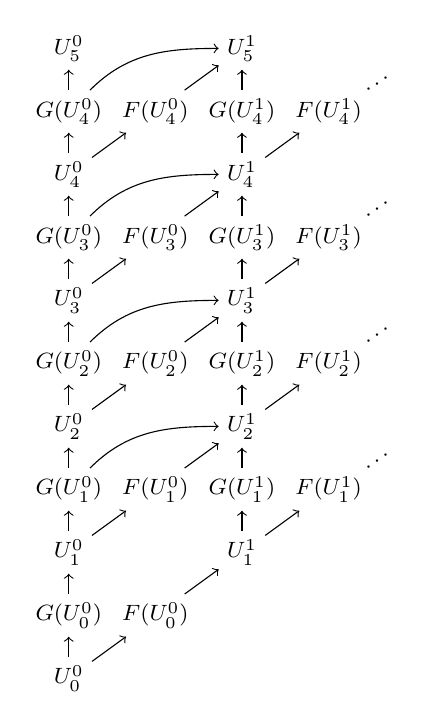
\begin{tikzpicture}[diag/.style={out=45,in=180}]
  \footnotesize
  \def\xshift{11mm}
  \def\yshift{8mm}
  \def\yangle{90}
  % initial value
  \action<+->{\pararealU{0}{0}}
  % k = 0, coarse solutions
  \foreach \n [evaluate={\nprev=int(\n-1)}] in {1,...,5} {%
  \action<+->{%
    \pararealG{\nprev}{0}
    \pararealU{\n}{0}
    \draw [->] (G\nprev0) -- (U\n0);
    \draw [->] (U\nprev0) -- (G\nprev0);
  }}
  % k = 0, fine solutions
  \action<+->{%
  \foreach \n in {0,...,4} {%
    \pararealF{\n}{0}
    \draw [->] (U\n0) -- (F\n0);
  }}
  % k = 0, transform to ghost
  \action<+->{}
  % k = 1, coarse solutions
  \action<+->{%
  \pararealU{1}{1}
  \draw [->] (F00) -- (U11);
  }
  \foreach \n [evaluate={\nprev=int(\n-1)}] in {2,...,5} {%
  \action<+->{%
    \pararealG{\nprev}{1}
    \pararealU{\n}{1}
    \draw [->] (G\nprev1) -- (U\n1);
    \draw [->] (F\nprev0) -- (U\n1);
    \draw [->] (G\nprev0) to [diag] (U\n1);
    \draw [->] (U\nprev1) -- (G\nprev1);
  }}
  % k = 1, fine solutions
  \action<+->{%
  \foreach \n in {1,...,4} {%
    \pararealF{\n}{1}
    \draw [->] (U\n1) -- (F\n1);
  }}
  % k = 2, coarse solutions
  %\action<+->{%
  %\pararealU{2}{2}
  %\draw [->] (F11) -- (U22);
  %\foreach \n [evaluate={\nprev=int(\n-1)}] in {3,...,5} {%
  %  \pararealG{\nprev}{2}
  %  \pararealU{\n}{2}
  %  \draw [->] (G\nprev2) -- (U\n2);
  %  \draw [->] (F\nprev1) -- (U\n2);
  %  \draw [->] (G\nprev1) to [diag] (U\n2);
  %  \draw [->] (U\nprev2) -- (G\nprev2);
  %}}
  % k = 2, fine solutions
  %\action<+->{%
  %\foreach \n in {2,...,4} {%
  %  \pararealF{\n}{2}
  %  \draw [->] (U\n2) -- (F\n2);
  %}}
  % rest
  \action<+->{%
  \foreach \n in {1,...,4} {%
    \draw (F\n1.north east)+(40:1ex) node [rotate=35] {$\cdots$};
  }}
\end{tikzpicture}
